% ****** Start of file aipsamp.tex ******
%
%   This file is part of the AIP files in the AIP distribution for REVTeX 4.
%   Version 4.1 of REVTeX, October 2009
%
%   Copyright (c) 2009 American Institute of Physics.
%
%   See the AIP README file for restrictions and more information.
%
% TeX'ing this file requires that you have AMS-LaTeX 2.0 installed
% as well as the rest of the prerequisites for REVTeX 4.1
%
% It also requires running BibTeX. The commands are as follows:
%
%  1)  latex  aipsamp
%  2)  bibtex aipsamp
%  3)  latex  aipsamp
%  4)  latex  aipsamp
%
% Use this file as a source of example code for your aip document.
% Use the file aiptemplate.tex as a template for your document.
\documentclass[%
 aip,
% jmp,
% bmf,
% sd,
% rsi,
 amsmath,amssymb,
%preprint,%
 reprint,%
%author-year,%
%author-numerical,%
% Conference Proceedings
]{revtex4-1}

\usepackage{graphicx}% Include figure files
\usepackage{dcolumn}% Align table columns on decimal point
\usepackage{bm}% bold math
%\usepackage[mathlines]{lineno}% Enable numbering of text and display math
%\linenumbers\relax % Commence numbering lines

\usepackage[utf8]{inputenc}
\usepackage[T1]{fontenc}
\usepackage{mathptmx}
\usepackage{etoolbox}

%% Apr 2021: AIP requests that the corresponding
%% email to be moved after the affiliations
\makeatletter
\def\@email#1#2{%
 \endgroup
 \patchcmd{\titleblock@produce}
  {\frontmatter@RRAPformat}
  {\frontmatter@RRAPformat{\produce@RRAP{*#1\href{mailto:#2}{#2}}}\frontmatter@RRAPformat}
  {}{}
}%
\makeatother
\begin{document}

\preprint{AIP/123-QED}

\title[Sample title]{Sample Title:\\with Forced Linebreak}
% Force line breaks with \\
\author{A. Author}
 \altaffiliation[Also at ]{Physics Department, XYZ University.}%Lines break automatically or can be forced with \\
\author{B. Author}%
 \email{Second.Author@institution.edu.}
\affiliation{
Authors' institution and/or address%\\This line break forced with \textbackslash\textbackslash
}%

\author{C. Author}
 \homepage{http://www.Second.institution.edu/~Charlie.Author.}
\affiliation{%
Second institution and/or address%\\This line break forced% with \\
}%

\date{\today}% It is always \today, today,
             %  but any date may be explicitly specified

\begin{abstract}
An article usually includes an abstract, a concise summary of the work
covered at length in the main body of the article. It is used for
secondary publications and for information retrieval purposes.
\end{abstract}

\maketitle

\begin{quotation}
The ``lead paragraph'' is encapsulated with the \LaTeX\
\verb+quotation+ environment and is formatted as a single paragraph before the first section heading. 
(The \verb+quotation+ environment reverts to its usual meaning after the first sectioning command.)
Note that numbered references are allowed in the lead paragraph.
%
The lead paragraph will only be found in an article being prepared for the journal \textit{Chaos}.
\end{quotation}

\section{\label{sec:level1}First-level heading:\protect\\ The line
break was forced \lowercase{via} \textbackslash\textbackslash}

This sample document demonstrates proper use of REV\TeX~4.1 (and
\LaTeXe) in manuscripts prepared for submission to AIP
journals. Further information can be found in the documentation included in the distribution or available at
\url{http://authors.aip.org} and in the documentation for
REV\TeX~4.1 itself.

When commands are referred to in this example file, they are always
shown with their required arguments, using normal \TeX{} format. In
this format, \verb+#1+, \verb+#2+, etc. stand for required
author-supplied arguments to commands. For example, in
\verb+\section{#1}+ the \verb+#1+ stands for the title text of the
author's section heading, and in \verb+\title{#1}+ the \verb+#1+
stands for the title text of the paper.

Line breaks in section headings at all levels can be introduced using
\textbackslash\textbackslash. A blank input line tells \TeX\ that the
paragraph has ended.

\subsection{\label{sec:level2}Second-level heading: Formatting}

This file may be formatted in both the \texttt{preprint} (the default) and
\texttt{reprint} styles; the latter format may be used to
mimic final journal output. Either format may be used for submission
purposes; however, for peer review and production, AIP will format the
article using the \texttt{preprint} class option. Hence, it is
essential that authors check that their manuscripts format acceptably
under \texttt{preprint}. Manuscripts submitted to AIP that do not
format correctly under the \texttt{preprint} option may be delayed in
both the editorial and production processes.

The \texttt{widetext} environment will make the text the width of the
full page, as on page~\pageref{eq:wideeq}. (Note the use the
\verb+\pageref{#1}+ to get the page number right automatically.) The
width-changing commands only take effect in \texttt{twocolumn}
formatting. It has no effect if \texttt{preprint} formatting is chosen
instead.

\subsubsection{\label{sec:level3}Third-level heading: Citations and Footnotes}

Citations in text refer to entries in the Bibliography;
they use the commands \verb+\cite{#1}+ or \verb+\onlinecite{#1}+.
Because REV\TeX\ uses the \verb+natbib+ package of Patrick Daly,
its entire repertoire of commands are available in your document;
see the \verb+natbib+ documentation for further details.
The argument of \verb+\cite+ is a comma-separated list of \emph{keys};
a key may consist of letters and numerals.

By default, citations are numerical; \cite{feyn54} author-year citations are an option.
To give a textual citation, use \verb+\onlinecite{#1}+: (Refs.~\onlinecite{witten2001,epr,Bire82}).
REV\TeX\ ``collapses'' lists of consecutive numerical citations when appropriate.
REV\TeX\ provides the ability to properly punctuate textual citations in author-year style;
this facility works correctly with numerical citations only with \texttt{natbib}'s compress option turned off.
To illustrate, we cite several together \cite{feyn54,witten2001,epr,Berman1983},
and once again (Refs.~\onlinecite{epr,feyn54,Bire82,Berman1983}).
Note that, when numerical citations are used, the references were sorted into the same order they appear in the bibliography.

A reference within the bibliography is specified with a \verb+\bibitem{#1}+ command,
where the argument is the citation key mentioned above.
\verb+\bibitem{#1}+ commands may be crafted by hand or, preferably,
generated by using Bib\TeX.
The AIP styles for REV\TeX~4 include Bib\TeX\ style files
\verb+aipnum.bst+ and \verb+aipauth.bst+, appropriate for
numbered and author-year bibliographies,
respectively.
REV\TeX~4 will automatically choose the style appropriate for
the document's selected class options: the default is numerical, and
you obtain the author-year style by specifying a class option of \verb+author-year+.

This sample file demonstrates a simple use of Bib\TeX\
via a \verb+\bibliography+ command referencing the \verb+aipsamp.bib+ file.
Running Bib\TeX\ (in this case \texttt{bibtex
aipsamp}) after the first pass of \LaTeX\ produces the file
\verb+aipsamp.bbl+ which contains the automatically formatted
\verb+\bibitem+ commands (including extra markup information via
\verb+\bibinfo+ commands). If not using Bib\TeX, the
\verb+thebibiliography+ environment should be used instead.

\paragraph{Fourth-level heading is run in.}%
Footnotes are produced using the \verb+\footnote{#1}+ command.
Numerical style citations put footnotes into the
bibliography\footnote{Automatically placing footnotes into the bibliography requires using BibTeX to compile the bibliography.}.
Author-year and numerical author-year citation styles (each for its own reason) cannot use this method.
Note: due to the method used to place footnotes in the bibliography, \emph{you
must re-run BibTeX every time you change any of your document's
footnotes}.

\section{Math and Equations}
Inline math may be typeset using the \verb+$+ delimiters. Bold math
symbols may be achieved using the \verb+bm+ package and the
\verb+\bm{#1}+ command it supplies. For instance, a bold $\alpha$ can
be typeset as \verb+$\bm{\alpha}$+ giving $\bm{\alpha}$. Fraktur and
Blackboard (or open face or double struck) characters should be
typeset using the \verb+\mathfrak{#1}+ and \verb+\mathbb{#1}+ commands
respectively. Both are supplied by the \texttt{amssymb} package. For
example, \verb+$\mathbb{R}$+ gives $\mathbb{R}$ and
\verb+$\mathfrak{G}$+ gives $\mathfrak{G}$

In \LaTeX\ there are many different ways to display equations, and a
few preferred ways are noted below. Displayed math will center by
default. Use the class option \verb+fleqn+ to flush equations left.

Below we have numbered single-line equations, the most common kind:
\begin{eqnarray}
\chi_+(p)\alt{\bf [}2|{\bf p}|(|{\bf p}|+p_z){\bf ]}^{-1/2}
\left(
\begin{array}{c}
|{\bf p}|+p_z\\
px+ip_y
\end{array}\right)\;,
\\
\left\{%
 \openone234567890abc123\alpha\beta\gamma\delta1234556\alpha\beta
 \frac{1\sum^{a}_{b}}{A^2}%
\right\}%
\label{eq:one}.
\end{eqnarray}
Note the open one in Eq.~(\ref{eq:one}).

Not all numbered equations will fit within a narrow column this
way. The equation number will move down automatically if it cannot fit
on the same line with a one-line equation:
\begin{equation}
\left\{
 ab12345678abc123456abcdef\alpha\beta\gamma\delta1234556\alpha\beta
 \frac{1\sum^{a}_{b}}{A^2}%
\right\}.
\end{equation}

When the \verb+\label{#1}+ command is used [cf. input for
Eq.~(\ref{eq:one})], the equation can be referred to in text without
knowing the equation number that \TeX\ will assign to it. Just
use \verb+\ref{#1}+, where \verb+#1+ is the same name that used in
the \verb+\label{#1}+ command.

Unnumbered single-line equations can be typeset
using the \verb+\[+, \verb+\]+ format:
\[g^+g^+ \rightarrow g^+g^+g^+g^+ \dots ~,~~q^+q^+\rightarrow
q^+g^+g^+ \dots ~. \]

\subsection{Multiline equations}

Multiline equations are obtained by using the \verb+eqnarray+
environment.  Use the \verb+\nonumber+ command at the end of each line
to avoid assigning a number:
\begin{eqnarray}
{\cal M}=&&ig_Z^2(4E_1E_2)^{1/2}(l_i^2)^{-1}
\delta_{\sigma_1,-\sigma_2}
(g_{\sigma_2}^e)^2\chi_{-\sigma_2}(p_2)\nonumber\\
&&\times
[\epsilon_jl_i\epsilon_i]_{\sigma_1}\chi_{\sigma_1}(p_1),
\end{eqnarray}
\begin{eqnarray}
\sum \vert M^{\text{viol}}_g \vert ^2&=&g^{2n-4}_S(Q^2)~N^{n-2}
        (N^2-1)\nonumber \\
 & &\times \left( \sum_{i<j}\right)
  \sum_{\text{perm}}
 \frac{1}{S_{12}}
 \frac{1}{S_{12}}
 \sum_\tau c^f_\tau~.
\end{eqnarray}
\textbf{Note:} Do not use \verb+\label{#1}+ on a line of a multiline
equation if \verb+\nonumber+ is also used on that line. Incorrect
cross-referencing will result. Notice the use \verb+\text{#1}+ for
using a Roman font within a math environment.

To set a multiline equation without \emph{any} equation
numbers, use the \verb+\begin{eqnarray*}+,
\verb+\end{eqnarray*}+ format:
\begin{eqnarray*}
\sum \vert M^{\text{viol}}_g \vert ^2&=&g^{2n-4}_S(Q^2)~N^{n-2}
        (N^2-1)\\
 & &\times \left( \sum_{i<j}\right)
 \left(
  \sum_{\text{perm}}\frac{1}{S_{12}S_{23}S_{n1}}
 \right)
 \frac{1}{S_{12}}~.
\end{eqnarray*}
To obtain numbers not normally produced by the automatic numbering,
use the \verb+\tag{#1}+ command, where \verb+#1+ is the desired
equation number. For example, to get an equation number of
(\ref{eq:mynum}),
\begin{equation}
g^+g^+ \rightarrow g^+g^+g^+g^+ \dots ~,~~q^+q^+\rightarrow
q^+g^+g^+ \dots ~. \tag{2.6$'$}\label{eq:mynum}
\end{equation}

A few notes on \verb=\tag{#1}=. \verb+\tag{#1}+ requires
\texttt{amsmath}. The \verb+\tag{#1}+ must come before the
\verb+\label{#1}+, if any. The numbering set with \verb+\tag{#1}+ is
\textit{transparent} to the automatic numbering in REV\TeX{};
therefore, the number must be known ahead of time, and it must be
manually adjusted if other equations are added. \verb+\tag{#1}+ works
with both single-line and multiline equations. \verb+\tag{#1}+ should
only be used in exceptional case - do not use it to number all
equations in a paper.

Enclosing single-line and multiline equations in
\verb+\begin{subequations}+ and \verb+\end{subequations}+ will produce
a set of equations that are ``numbered'' with letters, as shown in
Eqs.~(\ref{subeq:1}) and (\ref{subeq:2}) below:
\begin{subequations}
\label{eq:whole}
\begin{equation}
\left\{
 abc123456abcdef\alpha\beta\gamma\delta1234556\alpha\beta
 \frac{1\sum^{a}_{b}}{A^2}
\right\},\label{subeq:1}
\end{equation}
\begin{eqnarray}
{\cal M}=&&ig_Z^2(4E_1E_2)^{1/2}(l_i^2)^{-1}
(g_{\sigma_2}^e)^2\chi_{-\sigma_2}(p_2)\nonumber\\
&&\times
[\epsilon_i]_{\sigma_1}\chi_{\sigma_1}(p_1).\label{subeq:2}
\end{eqnarray}
\end{subequations}
Putting a \verb+\label{#1}+ command right after the
\verb+\begin{subequations}+, allows one to
reference all the equations in a subequations environment. For
example, the equations in the preceding subequations environment were
Eqs.~(\ref{eq:whole}).

\subsubsection{Wide equations}
The equation that follows is set in a wide format, i.e., it spans
across the full page. The wide format is reserved for long equations
that cannot be easily broken into four lines or less:
\begin{widetext}
\begin{equation}
{\cal R}^{(\text{d})}=
 g_{\sigma_2}^e
 \left(
   \frac{[\Gamma^Z(3,21)]_{\sigma_1}}{Q_{12}^2-M_W^2}
  +\frac{[\Gamma^Z(13,2)]_{\sigma_1}}{Q_{13}^2-M_W^2}
 \right)
 + x_WQ_e
 \left(
   \frac{[\Gamma^\gamma(3,21)]_{\sigma_1}}{Q_{12}^2-M_W^2}
  +\frac{[\Gamma^\gamma(13,2)]_{\sigma_1}}{Q_{13}^2-M_W^2}
 \right)\;. \label{eq:wideeq}
\end{equation}
\end{widetext}
This is typed to show the output is in wide format.
(Since there is no input line between \verb+\equation+ and
this paragraph, there is no paragraph indent for this paragraph.)
\section{Cross-referencing}
REV\TeX{} will automatically number sections, equations, figure
captions, and tables. In order to reference them in text, use the
\verb+\label{#1}+ and \verb+\ref{#1}+ commands. To reference a
particular page, use the \verb+\pageref{#1}+ command.

The \verb+\label{#1}+ should appear in a section heading, within an
equation, or in a table or figure caption. The \verb+\ref{#1}+ command
is used in the text where the citation is to be displayed.  Some
examples: Section~\ref{sec:level1} on page~\pageref{sec:level1},
Table~\ref{tab:table1},%
\begin{table}
\caption{\label{tab:table1}This is a narrow table which fits into a
text column when using \texttt{twocolumn} formatting. Note that
REV\TeX~4 adjusts the intercolumn spacing so that the table fills the
entire width of the column. Table captions are numbered
automatically. This table illustrates left-aligned, centered, and
right-aligned columns.  }
\begin{ruledtabular}
\begin{tabular}{lcr}
Left\footnote{Note a.}&Centered\footnote{Note b.}&Right\\
\hline
1 & 2 & 3\\
10 & 20 & 30\\
100 & 200 & 300\\
\end{tabular}
\end{ruledtabular}
\end{table}
and Fig.~\ref{fig:epsart}.

\section{Figures and Tables}
Figures and tables are typically ``floats''; \LaTeX\ determines their
final position via placement rules.
\LaTeX\ isn't always successful in automatically placing floats where you wish them.

Figures are marked up with the \texttt{figure} environment, the content of which
imports the image (\verb+\includegraphics+) followed by the figure caption (\verb+\caption+).
The argument of the latter command should itself contain a \verb+\label+ command if you
wish to refer to your figure with \verb+\ref+.

Import your image using either the \texttt{graphics} or
\texttt{graphix} packages. These packages both define the
\verb+\includegraphics{#1}+ command, but they differ in the optional
arguments for specifying the orientation, scaling, and translation of the figure.
Fig.~\ref{fig:epsart}%
\begin{figure}
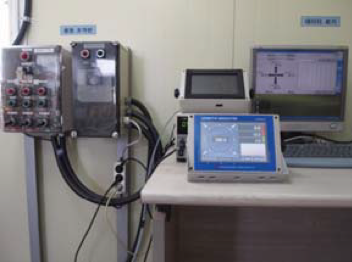
\includegraphics{fig_1}% Here is how to import EPS art
\caption{\label{fig:epsart} A figure caption. The figure captions are
automatically numbered.}
\end{figure}
is small enough to fit in a single column, while
Fig.~\ref{fig:wide}%
\begin{figure*}
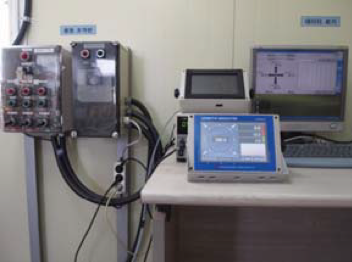
\includegraphics{fig_1}% Here is how to import EPS art
\caption{\label{fig:wide}Use the \texttt{figure*} environment to get a wide
figure, spanning the page in \texttt{twocolumn} formatting.}
\end{figure*}
is too wide for a single column,
so instead the \texttt{figure*} environment has been used.

The analog of the \texttt{figure} environment is \texttt{table}, which uses
the same \verb+\caption+ command.
However, you should type your caption command first within the \texttt{table},
instead of last as you did for \texttt{figure}.

The heart of any table is the \texttt{tabular} environment,
which represents the table content as a (vertical) sequence of table rows,
each containing a (horizontal) sequence of table cells.
Cells are separated by the \verb+&+ character;
the row terminates with \verb+\\+.
The required argument for the \texttt{tabular} environment
specifies how data are displayed in each of the columns.
For instance, a column
may be centered (\verb+c+), left-justified (\verb+l+), right-justified (\verb+r+),
or aligned on a decimal point (\verb+d+).
(Table~\ref{tab:table4}%
\begin{table}
\caption{\label{tab:table4}Numbers in columns Three--Five have been
aligned by using the ``d'' column specifier (requires the
\texttt{dcolumn} package).
Non-numeric entries (those entries without
a ``.'') in a ``d'' column are aligned on the decimal point.
Use the
``D'' specifier for more complex layouts. }
\begin{ruledtabular}
\begin{tabular}{ccddd}
One&Two&\mbox{Three}&\mbox{Four}&\mbox{Five}\\
\hline
one&two&\mbox{three}&\mbox{four}&\mbox{five}\\
He&2& 2.77234 & 45672. & 0.69 \\
C\footnote{Some tables require footnotes.}
  &C\footnote{Some tables need more than one footnote.}
  & 12537.64 & 37.66345 & 86.37 \\
\end{tabular}
\end{ruledtabular}
\end{table}
illustrates the use of decimal column alignment.)

Extra column-spacing may be be specified as well, although
REV\TeX~4 sets this spacing so that the columns fill the width of the
table.
Horizontal rules are typeset using the \verb+\hline+
command.
The doubled (or Scotch) rules that appear at the top and
bottom of a table can be achieved by enclosing the \texttt{tabular}
environment within a \texttt{ruledtabular} environment.
Rows whose columns span multiple columns can be typeset using \LaTeX's
\verb+\multicolumn{#1}{#2}{#3}+ command
(for example, see the first row of Table~\ref{tab:table3}).%
\begin{table*}
\caption{\label{tab:table3}This is a wide table that spans the page
width in \texttt{twocolumn} mode. It is formatted using the
\texttt{table*} environment. It also demonstrates the use of
\textbackslash\texttt{multicolumn} in rows with entries that span
more than one column.}
\begin{ruledtabular}
\begin{tabular}{ccccc}
 &\multicolumn{2}{c}{$D_{4h}^1$}&\multicolumn{2}{c}{$D_{4h}^5$}\\
 Ion&1st alternative&2nd alternative&lst alternative
&2nd alternative\\ \hline
 K&$(2e)+(2f)$&$(4i)$ &$(2c)+(2d)$&$(4f)$ \\
 Mn&$(2g)$\footnote{The $z$ parameter of these positions is $z\sim\frac{1}{4}$.}
 &$(a)+(b)+(c)+(d)$&$(4e)$&$(2a)+(2b)$\\
 Cl&$(a)+(b)+(c)+(d)$&$(2g)$\footnote{This is a footnote in a table that spans the full page
width in \texttt{twocolumn} mode. It is supposed to set on the full width of the page, just as the caption does. }
 &$(4e)^{\text{a}}$\\
 He&$(8r)^{\text{a}}$&$(4j)^{\text{a}}$&$(4g)^{\text{a}}$\\
 Ag& &$(4k)^{\text{a}}$& &$(4h)^{\text{a}}$\\
\end{tabular}
\end{ruledtabular}
\end{table*}

The tables in this document illustrate various effects.
Tables that fit in a narrow column are contained in a \texttt{table}
environment.
Table~\ref{tab:table3} is a wide table, therefore set with the
\texttt{table*} environment.
Lengthy tables may need to break across pages.
A simple way to allow this is to specify
the \verb+[H]+ float placement on the \texttt{table} or
\texttt{table*} environment.
Alternatively, using the standard \LaTeXe\ package \texttt{longtable}
gives more control over how tables break and allows headers and footers
to be specified for each page of the table.
An example of the use of \texttt{longtable} can be found
in the file \texttt{summary.tex} that is included with the REV\TeX~4
distribution.

There are two methods for setting footnotes within a table (these
footnotes will be displayed directly below the table rather than at
the bottom of the page or in the bibliography).
The easiest
and preferred method is just to use the \verb+\footnote{#1}+
command. This will automatically enumerate the footnotes with
lowercase roman letters.
However, it is sometimes necessary to have
multiple entries in the table share the same footnote.
In this case,
create the footnotes using
\verb+\footnotemark[#1]+ and \verb+\footnotetext[#1]{#2}+.
\texttt{\#1} is a numeric value.
Each time the same value for \texttt{\#1} is used,
the same mark is produced in the table.
The \verb+\footnotetext[#1]{#2}+ commands are placed after the \texttt{tabular}
environment.
Examine the \LaTeX\ source and output for Tables~\ref{tab:table1} and
\ref{tab:table2}%
\begin{table}
\caption{\label{tab:table2}A table with more columns still fits
properly in a column. Note that several entries share the same
footnote. Inspect the \LaTeX\ input for this table to see
exactly how it is done.}
\begin{ruledtabular}
\begin{tabular}{cccccccc}
 &$r_c$ (\AA)&$r_0$ (\AA)&$\kappa r_0$&
 &$r_c$ (\AA) &$r_0$ (\AA)&$\kappa r_0$\\
\hline
Cu& 0.800 & 14.10 & 2.550 &Sn\footnotemark[1]
& 0.680 & 1.870 & 3.700 \\
Ag& 0.990 & 15.90 & 2.710 &Pb\footnotemark[2]
& 0.450 & 1.930 & 3.760 \\
Au& 1.150 & 15.90 & 2.710 &Ca\footnotemark[3]
& 0.750 & 2.170 & 3.560 \\
Mg& 0.490 & 17.60 & 3.200 &Sr\footnotemark[4]
& 0.900 & 2.370 & 3.720 \\
Zn& 0.300 & 15.20 & 2.970 &Li\footnotemark[2]
& 0.380 & 1.730 & 2.830 \\
Cd& 0.530 & 17.10 & 3.160 &Na\footnotemark[5]
& 0.760 & 2.110 & 3.120 \\
Hg& 0.550 & 17.80 & 3.220 &K\footnotemark[5]
&  1.120 & 2.620 & 3.480 \\
Al& 0.230 & 15.80 & 3.240 &Rb\footnotemark[3]
& 1.330 & 2.800 & 3.590 \\
Ga& 0.310 & 16.70 & 3.330 &Cs\footnotemark[4]
& 1.420 & 3.030 & 3.740 \\
In& 0.460 & 18.40 & 3.500 &Ba\footnotemark[5]
& 0.960 & 2.460 & 3.780 \\
Tl& 0.480 & 18.90 & 3.550 & & & & \\
\end{tabular}
\end{ruledtabular}
\footnotetext[1]{Here's the first, from Ref.~\onlinecite{feyn54}.}
\footnotetext[2]{Here's the second.}
\footnotetext[3]{Here's the third.}
\footnotetext[4]{Here's the fourth.}
\footnotetext[5]{And etc.}
\end{table}
for an illustration.

All AIP journals require that the initial citation of
figures or tables be in numerical order.
\LaTeX's automatic numbering of floats is your friend here:
just put each \texttt{figure} environment immediately following
its first reference (\verb+\ref+), as we have done in this example file.

\begin{acknowledgments}
We wish to acknowledge the support of the author community in using
REV\TeX{}, offering suggestions and encouragement, testing new versions,
\dots.
\end{acknowledgments}

\section*{Data Availability Statement}

AIP Publishing believes that all datasets underlying the conclusions of the paper should be available to readers. Authors are encouraged to deposit their datasets in publicly available repositories or present them in the main manuscript. All research articles must include a data availability statement stating where the data can be found. In this section, authors should add the respective statement from the chart below based on the availability of data in their paper.

\begin{center}
\renewcommand\arraystretch{1.2}
\begin{tabular}{| >{\raggedright\arraybackslash}p{0.3\linewidth} | >{\raggedright\arraybackslash}p{0.65\linewidth} |}
\hline
\textbf{AVAILABILITY OF DATA} & \textbf{STATEMENT OF DATA AVAILABILITY}\\
\hline
Data available on request from the authors
&
The data that support the findings of this study are available from the corresponding author upon reasonable request.
\\\hline
Data available in article or supplementary material
&
The data that support the findings of this study are available within the article [and its supplementary material].
\\\hline
Data openly available in a public repository that issues datasets with DOIs
&
The data that support the findings of this study are openly available in [repository name] at http://doi.org/[doi], reference number [reference number].
\\\hline
Data openly available in a public repository that does not issue DOIs
&
The data that support the findings of this study are openly available in [repository name], reference number [reference number].
\\\hline
Data sharing not applicable – no new data generated
&
Data sharing is not applicable to this article as no new data were created or analyzed in this study.
\\\hline
Data generated at a central, large scale facility
&
Raw data were generated at the [facility name] large scale facility. Derived data supporting the findings of this study are available from the corresponding author upon reasonable request.
\\\hline
Embargo on data due to commercial restrictions
&
The data that support the findings will be available in [repository name] at [DOI link] following an embargo from the date of publication to allow for commercialization of research findings.
\\\hline
Data available on request due to privacy/ethical restrictions
&
The data that support the findings of this study are available on request from the corresponding author. The data are not publicly available due [state restrictions such as privacy or ethical restrictions].
\\\hline
Data subject to third party restrictions
&
The data that support the findings of this study are available from [third party]. Restrictions apply to the availability of these data, which were used under license for this study. Data are available from the authors upon reasonable request and with the permission of [third party].
\\\hline
\end{tabular}
\end{center}

\appendix

\section{Appendixes}

To start the appendixes, use the \verb+\appendix+ command.
This signals that all following section commands refer to appendixes
instead of regular sections. Therefore, the \verb+\appendix+ command
should be used only once---to set up the section commands to act as
appendixes. Thereafter normal section commands are used. The heading
for a section can be left empty. For example,
\begin{verbatim}
\appendix
\section{}
\end{verbatim}
will produce an appendix heading that says ``APPENDIX A'' and
\begin{verbatim}
\appendix
\section{Background}
\end{verbatim}
will produce an appendix heading that says ``APPENDIX A: BACKGROUND''
(note that the colon is set automatically).

If there is only one appendix, then the letter ``A'' should not
appear. This is suppressed by using the star version of the appendix
command (\verb+\appendix*+ in the place of \verb+\appendix+).

\section{A little more on appendixes}

Observe that this appendix was started by using
\begin{verbatim}
\section{A little more on appendixes}
\end{verbatim}

Note the equation number in an appendix:
\begin{equation}
E=mc^2.
\end{equation}

\subsection{\label{app:subsec}A subsection in an appendix}

You can use a subsection or subsubsection in an appendix. Note the
numbering: we are now in Appendix~\ref{app:subsec}.

\subsubsection{\label{app:subsubsec}A subsubsection in an appendix}
Note the equation numbers in this appendix, produced with the
subequations environment:
\begin{subequations}
\begin{eqnarray}
E&=&mc, \label{appa}
\\
E&=&mc^2, \label{appb}
\\
E&\agt& mc^3. \label{appc}
\end{eqnarray}
\end{subequations}
They turn out to be Eqs.~(\ref{appa}), (\ref{appb}), and (\ref{appc}).

\nocite{*}
\bibliography{aipsamp}% Produces the bibliography via BibTeX.

\end{document}
%
% ****** End of file aipsamp.tex ******
